\documentclass[reqno]{amsart}
\usepackage{amsfonts,amsmath,amsthm,amssymb,latexsym, cite}%
\usepackage{graphicx,verbatim}
\usepackage[colorlinks,plainpages,citecolor=magenta, linkcolor=blue ]{hyperref}%,bookmarksnumbered,, backref

\theoremstyle{plain}
\newtheorem{thm}{Theorem}
\newtheorem*{thrm}{Theorem}
\newtheorem{defn}{Definition}
\newtheorem{cor}{Corollary}
\newtheorem{lem}{Lemma}
\newtheorem{rem}{Remark}
\newtheorem{prop}{Proposition}


%\textwidth=125mm
%\textheight=195mm

\numberwithin{equation}{section}


\newcommand{\dom}{\mathop{\rm dom}}
\renewcommand{\Im}{\mathop{\rm Im}}
\newcommand{\supp}{\mathop{\rm supp}}
\newcommand{\sgn}{\mathop{\rm sgn}}
\newcommand{\rank}{\mathop{\rm rank}}
\renewcommand{\kappa}{\varkappa}
\newcommand{\rmi}{{\rm i}}
\newcommand{\Real}{\mathbb R}
\newcommand{\Cmpl}{\mathbb C}
\newcommand{\eps}{\varepsilon}
\newcommand{\en}{{\nu,\eps}}
\newcommand{\cI}{\mathcal{I}}
\newcommand{\cF}{\mathcal{F}}
\newcommand{\cE}{\mathcal{E}}
\newcommand{\mv}[1]{\langle #1 \rangle_0}
\newcommand{\fm}[1]{\langle #1 \rangle_1}
\newcommand{\fpr}[1]{{#1}^{(-1)}}
\newcommand{\spr}[1]{{#1}^{(-2)}}
\newcommand{\ra}{\rangle}
\newcommand{\la}{\langle}
\newcommand{\lme}{\lambda^\eps}

% MATH -----------------------------------------------------------
\newcommand{\norm}[1]{\left\Vert#1\right\Vert}
\newcommand{\abs}[1]{\left\vert#1\right\vert}
\newcommand{\set}[1]{\left\{#1\right\}}
\newcommand{\To}{\longrightarrow}
\newcommand{\BX}{\mathbf{B}(X)}
\newcommand{\A}{\mathcal{A}}
\newcommand{\cH}{\mathcal{H}}
\newcommand{\cV}{\mathcal{V}}
% ----------------------------------------------------------------

\newcommand{\mg}[1]{{\color{magenta}{#1}}}
\newcommand{\rd}[1]{{\color{red}{#1}}}
\renewcommand{\emph}[1]{{\textit{#1}}}
%\renewcommand{\phi}{\varphi}
\newcommand\rmd{\mathrm{d}}
\newcommand\rme{\mathrm{e}}
\newcommand\rmR{\mathrm{R}}
\renewcommand{\leq}{\leqslant}
\renewcommand{\geq}{\geqslant}
\newcommand{\myIm}{\mathop{\rm Im}}
\newcommand{\myRe}{\mathop{\rm Re}}
\newcommand{\sign}{\mathop{\rm sign}}
\newcommand{\ess}{\mathop{\rm ess}}
\newcommand{\bl}[1]{{\color{blue}{#1}}}
\newcommand{\oB}[1]{\langle{#1},g\rangle\hskip1pt f+\langle{#1},f\rangle\hskip1pt g}
\newcommand\nep{\textstyle\frac r\eps}
\newcommand\te{\left(\frac t\eps\right)}
\newcommand\se{\left(\frac s\eps\right)}
\newcommand\pfg{p}
\newcommand\hy{\hat{y}_\eps}
\newcommand{\pte}{\partial_n}
\newcommand{\pts}{\partial_s}
\newcommand{\npt}{\partial_\nu}

\begin{document}





\title[2D Schr\"{o}dinger operators with singular potentials]
{On spectra of 2D Schr\"{o}dinger operators with singular potentials localized in a neighbourhood of curve}





\author{Yuriy Golovaty}%
\address{Department of Mechanics and Mathematics,
  Ivan Franko National University of Lviv\\
  1 Universytetska str., 79000 Lviv, Ukraine}
\email{yuriy.golovaty@lnu.edu.ua}

\subjclass[2000]{Primary 34L40, 34B09; Secondary  81Q10}


\begin{abstract}
The
\end{abstract}


\keywords{}
\maketitle





%%%%%%%%%%%%%%%%%%%%%%%%%%%%%%%%%%%%%%%%%%%%%%%%%%%%%%%%%%%%%%%%%%%%%%%%%%
% Introduction
%%%%%%%%%%%%%%%%%%%%%%%%%%%%%%%%%%%%%%%%%%%%%%%%%%%%%%%%%%%%%%%%%%%%%%%%%%

\section{Introduction  }
\label{Sec:Introduction}




Throughout the paper, $W_2^m(\Omega)$ stands for the Sobolev space of functions defined on a set $\Omega$. $\sigma(A)$ is the spectrum







%%%%%%%%%%%%%%%%%%%%%%%%%%%%%%%%%%%%%%%%%%%%%%%%%%%%%%%%%%%%%%%%%%%%%%%%%%
% Statement of Problem and Main Results
%%%%%%%%%%%%%%%%%%%%%%%%%%%%%%%%%%%%%%%%%%%%%%%%%%%%%%%%%%%%%%%%%%%%%%%%%%

\section{Statement of Problem and Main Results}
\label{Sec:Statment}

We study the family of operators
\begin{equation}\label{OprHe}
H_\eps=-\Delta +W+V_\eps
\end{equation}
in $L_2(\Real^2)$, where the potential $W$ increases as $|x|\to +\infty$ and the perturbation $V_\eps$ has a compact support that shrinks to a curve as $\eps\to 0$. We define the family of potentials $V_\eps$ as follows.
Let $\gamma$ be a  closed  smooth curve without self-intersection
points. We will denote by $\omega_\eps$ the $\eps$-neighborhood of $\gamma$, i.e., the union of all open balls with the radius $\eps$ and a center on~$\gamma$.  Assume that the support of $V_\eps$ lies  in $\omega_\eps$. To specify  the explicit dependence of $V_\eps$ on  the small parameter $\eps$ we introduce  curvilinear coordinates  in $\omega_\eps$.
Let $\alpha\colon [0,m)\to \Real^2$, $\alpha=\alpha(s)$, be the unit-speed smooth parametrization of $\gamma$ with the natural parameter $s$, where $m$ is the length of $\gamma$.
Then the vector $\nu=(-\dot{\alpha}_2, \dot{\alpha}_1)$ is a unit normal on $\gamma$, because  $\dot{\alpha}_1^2+\dot{\alpha}_2^2=1$.
We define the local coordinates $(s,r)$ in $\omega_\eps$:
\begin{equation}\label{LocalTr}
    x=\alpha(s)+r\nu(s), \qquad (s,r)\in [0,m)\times (-\eps, \eps).
\end{equation}
The coordinate $r$ is the signed distance from a point $x$ to $\gamma$.
Suppose that the localized potential $V_\eps$ has the form
\begin{equation}\label{Veps}
V_\eps\big(\alpha(s)+r\nu(s)\big)=\eps^{-2}\,V\left(\eps^{-1}r\right)
+\eps^{-1}\,U\left(s,\eps^{-1}r\right),
\end{equation}
where $V$ and $U$ are smooth functions and  the supports
of $V$ and $U(s,\,\cdot\,)$ lie in the interval $\cI=(-1,1)$ for all $s$.
We note that the unperturbed operator $H_0=-\Delta +W$ is self-adjoint in $L^2(\Real^2)$ and its spectrum is discrete.  Obviously, the operator $H_\eps$ is also self-adjoint and  $\dom H_\eps=\dom H_0$.

\begin{figure}[t]
\centering
\includegraphics[scale=.6]{LocalCoords}
\caption{Curvilinear coordinates in the $\eps$-neighbourhood of $\gamma$.}
\label{FigLocalCoords}
\end{figure}


The family of potentials $V_\eps$ generally diverges in the space of distributions $\mathcal{D}(\Real^2)$.
As we will show  in Propositin~\ref{PropVepsConverg},
the  potentials converge only if $V$ is a zero mean function. In this case,
$V_\eps$ converges as $\eps\to 0$ to $a\partial_\nu\delta_\gamma+b\delta_\gamma$, where $a$ and $b$ are some functions on $\gamma$. The  distribution $\delta_\gamma$ is the Dirac delta function supported on the curve $\gamma$, and
\begin{equation*}
  \langle a\partial_\nu\delta_\gamma+b \delta_\gamma, \phi \rangle= -\int_\gamma  \npt(a\phi)\,d\gamma+\int_\gamma b \phi\,d\gamma\quad\text{for all }\phi\in C^\infty_0(\Real^2).
\end{equation*}
The main task is to describe the  asymptotic behaviour, as $\eps\to 0$, of the spectrum  of $H_\eps$, i.e., to construct the asymptotics of eigenvalues $\lambda^\eps$ and eigenfunctions $u_\eps$ of the spectral problem
\begin{equation}\label{SpectralEqn}
-\Delta u_\eps +(W+V_\eps) u_\eps= \lambda^\eps u_\eps\quad \hbox{in \ } \Real^2.
\end{equation}
Here and afterwards $\lambda^\eps$ stands for an eigenvalue of the operator $H_\eps$ and $u_\eps$ stands for the corresponding eigenfunction.




We  introduce some notation. The curve $\gamma$ divides the plane into two domains $\Omega^-$ and $\Omega^+$, i.e., $\Real^2=\Omega^-\cup\gamma\cup\Omega^+$. Suppose  $\Omega^+$ is unbounded.
Let us denote by $v^-$ and $v^+$ the one-side traces of $v$ on $\gamma$.

We  say that the Schr\"odinger operator~$-\frac{d^2}{d t^2}+V$ in $L_2(\Real)$ possesses a \emph{zero-energy resonance}  if there exists a non trivial solution~$h$ of the equation $-h'' +Vh= 0$ that is bounded on the whole line.  We call $h$ the \emph{half-bound state}.  Such a solution~$h$ is  unique up to a scalar factor and has nonzero limits
\begin{equation*}
  h(-\infty)=\lim\limits_{t\to-\infty}h(t), \qquad
  h(+\infty)=\lim\limits_{t\to+\infty}h(t).
\end{equation*}

Let $\cE\subset(0, 1)$ be an infinite set, for which zero is an accumulation point.
Our main result reads as follows.


\begin{thm}\label{MainThrmRes}
Assume that the Schr\"odinger operator~$-\frac{d^2}{d t^2}+V$ in $L_2(\Real)$ possesses a zero-energy resonance with the half-bound state $h$.

(i) Suppose that $\{\lme\}_{\eps\in\cE}$ is a sequence of eigenvalues of $H_\eps$ and $\{u_\eps\}_{\eps\in\cE}$ is the corresponding sequence of  eigenfunctions such that $\|u_\eps\|_{L_2(\Real^2)}=1$. If
\begin{equation}\label{LmneToLmn}
  \lme \to \lambda, \qquad u_\eps \to u\quad \text{in } L_2(\Real^2) \   \text{weakly}
\end{equation}
as $\cE\ni\eps\to 0$,  and $u$ is a non-zero function, then $\lambda$ and $u$ are an eigenvalue and the corresponding eigenfunction of the operator $\cH=-\Delta +W$ acting on the domain
\begin{align*}
  \dom \cH=\big\{v\in W_2^2&(\Omega\setminus\gamma)\colon\;v^+-\theta v^-=0,\\  &\theta\partial_\nu v^+-\partial_\nu v^-
=\left(\textstyle\frac{1}{2 }(\theta^2-1)\kappa+\mu\right) v^-\,\text{on } \gamma \big\}.
\end{align*}
Here $\theta=h(+\infty)/h(-\infty)$, $\kappa=\kappa(s)$ is the  curvature of $\gamma$, and
\begin{equation}\label{Mu}
  \mu(s)=\frac{1}{h^2(-\infty)} \int_{\cI} U(s,r)h^2(r)\, dr,\quad s\in [0,m).
\end{equation}

(ii) If \eqref{LmneToLmn} holds and $\lambda$ is not a point of  $\sigma(\cH)$, then the sequence of eigenfunctions $u_\eps$ converges to zero as $\eps\to 0$ in the weak topology of  $L_2(\Real^2)$.

(iii) For each eigenvalue $\lambda$ of the operator $\cH$ and  all $\eps$ small enough there exists an eigenvalue $\lme$ of the operator $H_\eps$ such that
$|\lme-\lambda|\leq c\eps$
with the constant $c$ depending only on $\lambda$.
\end{thm}

The trivial potential $V=0$ possesses a zero-energy resonance with a constant function as  the half-bound state. Then $V_\eps(x) =\eps^{-1}\,U\left(s,\eps^{-1}n\right)$ and
$V_\eps\to \mu_0 \delta_\gamma$ as $\eps\to 0$ in the space of distributions, where
\begin{equation}\label{Mu0}
  \mu_0(s)=\int_{\cI}U(s,t)\, dt,\qquad s\in [0,m).
\end{equation}
Moreover the parameter $\theta$ equals  $1$ and the interface conditions
\begin{equation}\label{ConnectedCond}
  v^+-\theta v^-=0,\quad \theta\partial_\nu v^+-\partial_\nu v^-
=\left(\textstyle\frac{1}{2 }(\theta^2-1)\kappa+\mu\right) v^-
\end{equation}
on the curve  $\gamma$ become
\begin{equation*}
  v^+- v^-=0, \quad \partial_\nu v^+-\partial_\nu v^-
=\mu_0 v^-.
\end{equation*}
The last conditions are exactly the same as that obtained in \cite{BehrndtExnerHolzmannLotoreichik2017}.





Let us introduce two operators
\begin{equation*}
  \mathcal{D}^\pm= -\Delta+W\quad\text{in }L_2(\Omega^\pm), \qquad \dom \mathcal{D}^\pm=\{v\in W_2^2(\Omega^\pm)\colon\; v=0 \;\,\mbox{on } \gamma\}.
\end{equation*}


\begin{thm}\label{MainThrmNoRes}
Suppose that the Schr\"odinger operator~$-\frac{d^2}{d t^2}+V$ in $L_2(\Real)$ has no zero-energy resonance.

 (i) If $\lme \to \lambda$ and $u_\eps \to u$ in $L_2(\Real^2)$ weakly, as $\cE\ni\eps\to 0$, and the limit function $u$ is different from zero, then
$\lambda$ is an eigenvalue of the direct sum $\mathcal{D}^-\oplus\mathcal{D}^+$ and $u$ is the corresponding eigenfunction.


(ii) In the case that $\lme \to \lambda$ and $\lambda\not\in \sigma(\mathcal{D}^-\oplus\mathcal{D}^+)$, the eigenfunctions $u_\eps$ converge to zero in $L_2(\Real^2)$ weakly.

(iii) If $\lambda\in \sigma(\mathcal{D}^-\oplus\mathcal{D}^+)$, then for all $\eps$ small enough we can find  an eigenvalue $\lme$ of $H_\eps$ such that
$ |\lme-\lambda|\leq c\eps$,
where the constant $c$ does not depend on $\eps$.
\end{thm}




The thin structure that is the singular potential $V_\eps$ can produce a series of negative eigenvalues which go to the negative infinity as $\eps\to 0$ (see Fig.~\ref{FigSpectrum}). Although for each $\eps>0$ the number of negative eigenvalues is finite, for some potentials $V_\eps$ this number can increase infinitely as $\eps\to 0$.  In particular, this means that the family of operators $H_\eps$ is not uniformly bounded from below with respect to the small parameter $\eps$.

In the case of such spectrum behavior, each real point $\lambda$ can be realized as an accumulation point of the eigenvalues $\lme$ of $H_\eps$,  as $\eps\to 0$. In Fig.~\ref{FigSpectrum}, we see that the dashed line beginning at a point $\lambda$ has infinitely many intersections with curves $\lme$.
Theorems~\ref{MainThrmRes} and  \ref{MainThrmNoRes} point out the basic difference between the points of the spectra of  limit operators and all other ones. This difference is that only the points of $\sigma(\cH)$ in the resonant case (or $\sigma(\mathcal{D}^-\oplus\mathcal{D}^+)$ in the non-resonant case) can be approximated by $\lme$ so that the corresponding eigenfunctions $u_\eps$  have a nontrivial limit.
In a particular case, the result of Theorem~\ref{MainThrmNoRes} can be improved.

\begin{thm}\label{MainThrmVUPos}
Assume that the potentials $V$ and $U$ in \eqref{Veps} are non-negative.
Then $\lme \to \lambda$  as $\eps\to 0$ if and only if $\lambda$ is an eigenvalue of the direct sum $\mathcal{D}^-\oplus\mathcal{D}^+$. In addition,  the corresponding eigenfunctions $u_\eps$ converge in the $L_2$-norm to an eigenfunction $u$ associated with the eigenvalue $\lambda$.
\end{thm}








%%%%%%%%%%%%%%%%%%%%%%%%%%%%%%%%%%%%%%%%%%%%%%%%%%%%%%%%%%%%%%%%%%%%%%%%%%
% Preliminaries
%%%%%%%%%%%%%%%%%%%%%%%%%%%%%%%%%%%%%%%%%%%%%%%%%%%%%%%%%%%%%%%%%%%%%%%%%%

\section{Preliminaries}
Returning  to the curvilinear coordinates $(s,r)$ given by \eqref{LocalTr},
we see that the couple of vectors
$ \alpha=(\dot{\alpha}_1, \dot{\alpha}_2)$, $\nu=(-\dot{\alpha}_2, \dot{\alpha}_1)$
gives a Frenet frame for $\gamma$.
The Jacobian of transformation $x=\alpha(s)+r\nu(s)$ has the form
\begin{multline*}
J(s,r)=
\begin{vmatrix}
  \dot{\alpha}_1(s)-r\ddot{\alpha}_2(s)& -\dot{\alpha}_2(s)\\
          \dot{\alpha}_2(s)+r\ddot{\alpha}_1(s)\phantom{0} & \dot{\alpha}_1(s)
\end{vmatrix}
\\
=\dot{\alpha}_1^2(s)+\dot{\alpha}_2^2(s)
-r\big(\dot{\alpha}_1(s)\ddot{\alpha}_2(s)-
  \dot{\alpha}_2(s)\ddot{\alpha}_1(s)\big)=1-r \kappa(s),
\end{multline*}
where $\kappa=\det(\dot{\alpha},\ddot{\alpha})$ is the signed curvature of $\gamma$.
We see that $J$ is positive for sufficiently small $r$, because  curvature $\kappa$  is  bounded on $\gamma$.
Namely, the curvilinear coordinates $(s,r)$ can be defined correctly on  $\omega_\eps$ for all $\eps<\eps_*$, where
\begin{equation}\label{EpsStar}
	\eps_*=\min_{\gamma}|\kappa|^{-1}.
\end{equation}
Note also that $\kappa$ is defined uniquely up to the re-parametrization $s\mapsto-s$.
Interface conditions \eqref{ConnectedCond} contain the parameters $\theta$, $\kappa$ and $\mu$ which depend on the particular parametrization chosen for curve $\gamma$, i.e., the parameters change along with the change of the Frenet frame.

\begin{prop}\label{PropInvarianceOfCnds}
  Operator $\mathcal{H}$ in Theorem~\ref{MainThrmRes} does not depend upon the choice of the Frenet frame for  $\gamma$.
\end{prop}
\begin{proof}
Every smooth curve  admits two possible orientations of the arc-length parameter and consequently two possible  Frenet frames. Let us change the Frenet frame $\{\alpha, \nu\}$ to the frame $\{-\alpha, -\nu\}$ and prove that interface conditions \eqref{ConnectedCond} will remain the same. This change leads to the following transformations:
\begin{equation*}
h(\pm\infty)\mapsto h(\mp\infty),\;\;
\theta\mapsto \theta^{-1}, \;\; \kappa\mapsto -\kappa,\;\; \mu\mapsto \theta^{-2}\mu, \;\; u_\pm\mapsto u_\mp, \;\; \partial_\nu u_\pm \mapsto -\partial_\nu u_\mp.
\end{equation*}
The first condition $u^+-\theta u^-=0$ in \eqref{ConnectedCond} transforms into $u^--\theta^{-1} u^+=0$ and therefore remains unchanged. For the second condition, we obtain
\begin{equation*}
 	-\theta^{-1}\partial_\nu u^-+\partial_\nu u^+
	-\left(-\textstyle\frac{1}{2}(\theta^{-2}-1)\kappa
	+\theta^{-2}\mu\right) u^+=0.
\end{equation*}
Multiplying the equality by $\theta$  yields
\begin{equation*}
	\theta\partial_\nu u^+-\partial_\nu u^-
	-\left(\textstyle\frac{1}{2 }(\theta^{2}-1)\kappa+\mu\right) 	\theta^{-1} u^+=0,
\end{equation*}
since $-\theta(\theta^{-2}-1)=\theta^{-1}(\theta^{2}-1)$. It remains to insert $u^-$ in place of $\theta^{-1} u^+$, in view of the first interface condition.
\end{proof}





The metric tensor $g=(g_{ij})$ in the orthogonal coordinates $(s,r)$  has the form
  \begin{equation*}
    g=
    \begin{pmatrix}
      J^2\phantom{0} & 0 \\
          0\phantom{0} & 1
    \end{pmatrix}.
  \end{equation*}
In fact, we have
$g_{11}=|x_s|^2=|\dot{\alpha}+r \dot{\nu}|^2
=|(1-r\kappa) \dot{\alpha}|^2=J^2$,
by the Frenet-Serret formula $\dot{\nu}=-\kappa \dot{\alpha}$, and $g_{22}=|x_r|^2=|\nu|^2=1$.
In particular,  the  Laplace-Beltrami operator in $\omega_\eps$ has  the form
\begin{equation}\label{LaplacianInSN}
\Delta \phi=J^{-1}\left(\partial_s(J^{-1}\partial_s \phi)+ \partial_r(J\partial_r \phi)\right).
\end{equation}




All the results presented in Theorems~\ref{MainThrmRes} and~\ref{MainThrmNoRes}  concern arbitrary potentials $V_\eps$ of the form \eqref{Veps} that generally diverge in the distributional sense. However,  the spectra of $H_\eps$ converge to spectra of the limit operators  without reference to the convergence of the potentials. The following statement shows that the convergence conditions for the potentials $V_\eps$ and the spectra of $H_\eps$ are quite different.

\begin{prop}\label{PropVepsConverg}
The family of potentials $V_\eps$ converges in the space of distributions $\mathcal{D}'(\Real^2)$ if and only if $V$ is a zero mean function, i.e.,
$\int_\Real V\,dt=0$. In this case,
\begin{equation*}
  V_\eps\to \beta\,\partial_\nu\delta_\gamma+\left(\beta\kappa+\mu_0\right) \delta_\gamma \quad \text{in }\mathcal{D}'(\Real^2),
\end{equation*}
where $\beta=-\int_\Real r V(r)\,dr$ and $\mu_0$ is given by \eqref{Mu0}.
\end{prop}
\begin{proof}
It is evident that the sequence $\eps^{-1}\,U\left(s,\eps^{-1}r\right)$
converge to  $\mu_0 \delta_\gamma$ in $\mathcal{D}'(\Real^2)$.
Write $g_\eps=\eps^{-2}\,V\left(\eps^{-1}r\right)$  and $n=\eps^{-1}r$. Then we have
\begin{multline*}
\int_{\Real^2}g_\eps\phi\,dx
=\int_{\omega_\eps}g_\eps\phi\,dx
=
\eps^{-2}\int_{-\eps}^\eps\int_{0}^m V(\eps^{-1}r)\phi(s,r)(1-r\kappa(s))\,ds\,dr
\\
 =
\eps^{-1}\int_{-1}^1\int_0^m V(n)\phi(s,\eps n)(1-\eps n\kappa(s))\,ds\,dn
=\eps^{-1}\int_{-1}^1 V(n)\,dn \int_0^m\phi(s,0)\,ds
\\
+
\int_{-1}^1 n V(n)\,dn \int_0^m\big(\partial_n\phi(s,0)-\kappa(s)\phi(s,0)\big)\,ds+O(\eps)
\end{multline*}
as $\eps\to 0$  for all $\phi\in C^\infty_0(\Real^2)$.
The  sequence $g_\eps$ has a finite limit as $\eps\to 0$ in $\mathcal{D}'(\Real^2)$ iff $\int_\Real V\,dt=0$.
In this case, we have
\begin{equation*}
\int_{\Real^2}g_\eps\phi\,dx\to \beta\int_\gamma\left(\partial_\nu\delta_\gamma+\kappa \delta_\gamma\right)\phi\,d\gamma,
\end{equation*}
which completes the proof.
\end{proof}







%%%%%%%%%%%%%%%%%%%%%%%%%%%%%%%%%%%%%%%%%%%%%%%%%%%%%%%%%%%%%%%%%%%%%%%%%%
% Calculation of Limit Operator
%%%%%%%%%%%%%%%%%%%%%%%%%%%%%%%%%%%%%%%%%%%%%%%%%%%%%%%%%%%%%%%%%%%%%%%%%%

\section{Formal Asymptotics of Eigenvalues}\label{Sec:LimitOperator}

Now we will show how interface conditions \eqref{ConnectedCond} can be found by direct calculations, constructing the formal asymptotics of  eigenvalues and eigenfunctions.

In the sequel, the normal vector field $\nu$ on $\gamma$ will be outward to domain $\Omega^-$, that is to say, the local coordinate $r$ will increase in the direction from $\Omega^-$ to $\Omega^+$. We also denote by $\gamma_t=\{x\in\Real^2\colon\; x=\alpha(s)+t\nu(s), \; s\in S\}$ the closed curve that is obtained from $\gamma$ by flowing for ``time'' $t$ along the normal vector field. Then the boundary of $\omega_\eps$ consists of two curves $\gamma_{-\eps}$ and $\gamma_{\eps}$.

We  look for the  approximation to an eigenvalue $\lambda_\eps$ and the corresponding eigenfunction $u_\eps$ of \eqref{SpectralEqn} in the form
\begin{equation}\label{AsymptoticsUe}
\lambda^\eps\approx \lambda, \qquad u_\eps(x)\approx
\begin{cases}
  u(x)& \hbox{in \ }\Real^2\setminus \omega_\eps, \\
    v_0\left(s,\nep\right)+\eps v_1\left(s,\nep\right)+\eps^2 v_2\left(s,\nep\right)
&\hbox{in \ } \omega_\eps.
\end{cases}
\end{equation}
To match the approximations in $\omega_\eps$ and $\Real^2\setminus \omega_\eps$, we hereafter assume that
\begin{equation}\label{MatchingCnds}
  [u_\eps]_{\pm\eps}=0, \quad [\partial_r u_\eps]_{\pm\eps}=0,
\end{equation}
where  $[w]_t$ stands for  the jump of $w$ across $\gamma_t$ in the positive direction of the local coordinate $r$.


Since the function $u_\eps$ solves \eqref{SpectralEqn} and the domain $\omega_\eps$ shrinks to $\gamma$, the function $u$ must be a solution of the equation
\begin{equation*}
-\Delta u+Wu= \lambda u \quad \hbox{in \ } \Real^2\setminus \gamma,
\end{equation*}
subject to appropriate interface conditions on $\gamma$.
To find these conditions, we consider equation \eqref{SpectralEqn} in the curvilinear coordinates $(s,n)$, where $n=r/\eps$. Here and afterwards it will be convenient to parameterize the curve $\gamma$ by the points of a circle. This  will allow us not to indicate every time that the functions $v_k=v_k(s,n)$ are periodic with respect to $s$.
Let $S$ be the circle of the same length as the length of $\gamma$.
Then $\omega_\eps$ is diffeomorphic to the cylinder $Q_\eps=S\times (-\eps, \eps)$ for $\eps$ small enough. Given a point $x\in \omega_\eps$, we write
\begin{equation*}
    x=\alpha(s)+r\nu(s), \qquad (s,r)\in S\times (-\eps, \eps).
\end{equation*}
We also set  $Q=S\times \cI$.
In the vicinity of $\gamma$ the Laplacian can be written as
\begin{equation*}
  \Delta =\frac1{1-\eps n\kappa}\left( \eps^{-2}\partial_n
  (1-\eps n\kappa)\partial_n +\partial_s
  \Big(\frac1{1-\eps n\kappa}\,\partial_s\Big)\right),
\end{equation*}
by \eqref{LaplacianInSN}.
From this we readily deduce the  representation
\begin{equation}\label{LaplaceExpansion}
\Delta= \eps^{-2}\partial^2_n-\eps^{-1}\kappa(s)\partial_n
-n\kappa^2(s)\partial_n+\partial^2_s+\eps P_\eps,
\end{equation}
where $P_\eps$ is a partial differential operator of the second order on $s$ and the first one on $n$ whose coefficients  are uniformly bounded in $Q$ with respect to $\eps$.


Substituting \eqref{AsymptoticsUe} into \eqref{SpectralEqn} for $x\in \omega_\eps$ in particular yields
\begin{equation}\label{EqnsV0V1}
-\pte^2 v_0+V(n)v_0=0,
\qquad
-\pte^2 v_1+V(n)v_1=-\kappa(s)\pte v_0-U(s,n)v_0
\end{equation}
\begin{equation}\label{EqnV2}
  -\pte^2 v_2+V(n)v_2=-(\kappa(s)\pte +U(s,n)) v_1\\
  +(\partial^2_s-n\kappa^2\partial_n-W(s,0)+\lambda)v_0
\end{equation}
in the cylinder $Q$.
From \eqref{MatchingCnds} we see that necessarily
\begin{gather}\label{FittingCndsUV0}
 u^-(s)=v_0(s,-1),\qquad u^+(s)=v_0(s,1),
 \\\label{FittingCndspV0}
 \partial_n v_0(s,- 1)=0, \qquad \partial_n v_0(s, 1)=0, \\\label{FittingCndspV1}
 \partial_n v_1(s, -1)=\partial_r u^-(s), \qquad
 \partial_n v_1(s, 1)=\partial_r u^+(s),
\end{gather}
where $u^\pm$ are the one-side traces of $u$ on $\gamma$.
Combining \eqref{FittingCndspV0}--\eqref{FittingCndspV1}, we conclude that $v_0$ and $v_1$ solve the boundary value problems
\begin{align}\label{problemV0}
&\begin{cases}
  -\pte^2 v_0+V(n)v_0=0 \quad \hbox{in \ } Q, \\
    \phantom{-}\partial_n v_0(s,- 1)=0, \quad \partial_n v_0(s, 1)=0, \quad s\in S;
\end{cases}
\\\label{problemV1}
&\begin{cases}
  -\pte^2 v_1+V(n)v_1=-\kappa(s)\pte v_0-U(s,n)v_0\quad \hbox{in \ } Q, \\
    \phantom{-}\partial_n v_1(s, -1)=\partial_r u^-(s), \quad
\partial_n v_1(s, 1)=\partial_r u^+(s), \quad s\in S
\end{cases}
\end{align}
respectively. Hence we have the boundary value problems for the ``non-ellip\-tic'' partial differential operator $-\pte^2+V$ in the cylinder $Q$. These problems can also be  regarded as  boun\-da\-ry value problems for ordinary differential equations on $\cI$ which depend on the parameter $s\in S$.


\subsection{Case of zero-energy resonance}
Assume that operator $-\frac{d^2}{dt^2}+V$ has a zero energy resonance with half-bound state $h$. Since the support of $V$ lies in  the interval $\cI$, the half-bound state $h$ is  constant  outside $\cI$ as a bounded solution of the equation $h''=0$.
Therefore the restriction of $h$ to $\cI$ is a nonzero solution of the Neumann boundary value problem
\begin{equation}\label{NeumanProblem}
     -h''+V(n)h=0 \text{ \ in }\cI,\qquad   h'(-1)=0, \quad h'(1)=0.
\end{equation}
Hereafter, we fix $h$ by additional condition $h(-1)=1$. Then $h(\pm\infty)=h(\pm 1)$ and $\theta=h(1)$.
In this case, \eqref{problemV0}  admits a infinitely many solutions $v_0(s,n)=a_0(s)h(n)$, where $a_0$ is an arbitrary function on $S$.
From \eqref{FittingCndsUV0} we deduce that $u^-=a_0$ and $u^+=h(1) a_0=\theta a_0$ and hence that $v_0(s,n)=u^-(s)h(n)$ and
\begin{equation}\label{RCond0}
     u^+=\theta u^-\quad\text {on }\gamma.
\end{equation}



Next, problem \eqref{problemV1} is in general unsolvable, since \eqref{problemV0} admits  nontrivial solutions.  To find solvabi\-li\-ty conditions, we rewrite  equation in \eqref{problemV1} in the form
\begin{equation}\label{eqnV1Expand}
  -\pte^2 v_1+V(n)v_1=-\big(\kappa(s)h'(n)+U(s,n)h(n)\big)u^-(s),
\end{equation}
multiply  by $a(s)h(n)$, $a\in L^2(S)$,  and then integrate over $Q$
\begin{multline}\label{IntV1H}
\int_{Q}\left(-\pte^2 v_1+V(n)v_1\right)a(s)h(n)\,dn\,ds
\\
=
-\int_{Q}(\kappa(s)h'(n)+U(s,n)h(n))u^-(s)a(s)h(n)\, dn\,ds.
\end{multline}
Since $h$ is a solution of \eqref{NeumanProblem}, integrating by parts twice on the left-hand side yields
\begin{multline*}
\int_{S} \int_{\cI}\left(-\pte^2 v_1+Vv_1\right)a h\,dn \,ds
=-\int_{S}( \partial_n v_1 h-v_1 h')\big|_{n=-1}^{n=1}a\,ds\\-
\int_{S} \int_{\cI} a v_1\left(-h''+Vh\right)\,dn\,ds
=-\int_{S}\big(\theta\partial_r u^+-\partial_r u^-\big) a\,ds,
\end{multline*}
in view of the boundary conditions for $v_1$.
Hence \eqref{IntV1H} becomes
\begin{equation*}
\int_{S}\left(\theta\partial_r u^+-\partial_r u^-\right)a\,ds
=\int_{S} u^-a\int_{\cI}\left(\kappa hh'+U h^2\right)\,dn\,ds.
\end{equation*}
The equality  $hh'=\frac12 (h^2)'$ implies
\begin{equation}\label{IntHHpr}
\int_{\cI}hh'\,dn=\tfrac12 (h^2(1)-h^2(-1))=\tfrac{1}{2 }(\theta^2-1).
\end{equation}
 Therefore we obtain
\begin{equation*}
\int_{S}\left(\theta\partial_r u^+-\partial_r u^-\right)a\,ds
=\int_{S}\big(\textstyle\frac{1}{2}(\theta^2-1)\kappa+\mu \big)u^-a\,ds
\end{equation*}
for all  $a\in L^2(S)$, where $\mu(s)=\int_{\cI} U(s,n)h^2(n)\, dn$.
From this we deduce
\begin{equation*}
  \theta\partial_r u^+-\partial_r u^-
=\big(\textstyle\frac{1}{2}(\theta^2-1)\kappa+\mu \big) u^-\quad\text {on }\gamma,
\end{equation*}
which is necessary for the solvability of \eqref{problemV1}.
In view of the Fredholm alternative, this condition is also  sufficient. Moreover it is a jump condition for the normal derivative of $u$   at the interface $\gamma$, since $\partial_\nu=\partial_r$ on $\gamma$.

Therefore  $\lambda$ and $u$ in the approximation \eqref{AsymptoticsUe} must solve the problem
\begin{gather}\label{LimitProblemEq}
-\Delta u+Wu=\lambda u \qquad \hbox{in  } \Real^2\setminus \gamma,
\\ \label{RConds}
 \phantom{-}u^+-\theta u^-=0,  \quad
\theta\partial_\nu u^+-\partial_\nu u^-
=\big(\textstyle\frac{1}{2}(\theta^2-1)\kappa+\mu \big) u^- \quad \hbox{on } \gamma,
\end{gather}
i.e., the spectral equation $\cH u=\lambda u$. 
Assume that $\lambda$ is an eigenvalue of operator $\cH$ and $u$  is an eigenfunction for this eigenvalue.

Now we can calculated the trace $u^-$ on $\gamma$ and  finally determine $v_0(s,n)=u^-(s)h(n)$.

Since the second condition in \eqref{RConds} holds,
problem \eqref{problemV1} is solvable and $v_1$ is defined up to the term $a_1(s) h(n)$.
Choose the solution $v_1$ so that $v_1(s,-1)=0$ for all $s\in S$.
We also suppose that $v_2$ solves the Cauchy problem
\begin{align}
&\begin{aligned}\label{problemV2eqn}
  -\pte^2 v_2+V(n)v_2=-(\kappa(s)&\pte +U(s,n)) v_1\\
  &+(\partial^2_s-n\kappa^2\partial_n-W(s,0)+\lambda)v_0
  \quad \hbox{in \ } Q,
\end{aligned}
\\\label{problemV2conditions}
 & \phantom{-} v_2(s, -1)=0,
 \quad
 \partial_n v_2(s, -1)=0, \quad s\in S.
\end{align}



\subsection{Non-resonant case}
Now suppose that problem \eqref{NeumanProblem} admits the trivial solution only.  Then $v_0=0$ and therefore $u^-=0$ and $u^+=0$ on $\gamma$, by \eqref{FittingCndsUV0}. We thus get
\begin{equation*}
-\Delta u+Wu=\lambda u\quad \hbox{in \ } \Real^2\setminus \gamma,\qquad
 u|_{\gamma}=0.
\end{equation*}
Let us suppose that $\lambda$ is an eigenvalue of the direct sum
$\mathcal{D}_1\oplus\mathcal{D}_2$ of two Dirichlet type operators and $u$ is a corresponding eigenfunction.
In this case, problem \eqref{problemV1} has the form
\begin{equation}\label{problemV1Non}
\begin{cases}
    -\pte^2 v_1+V(n)v_1=0\quad \hbox{in \ } Q, \\
    \phantom{-}\partial_n v_1(s, -1)=\partial_\nu u^-, \qquad
\partial_n v_1(s, 1)=\partial_\nu u^+,
\end{cases}
\end{equation}
and admits a unique solution. We also assume that
\begin{equation*}
\begin{cases}
-\pte^2 v_2+V(n)v_2=-\kappa(s)\pte v_1 +U(s,n) v_1
  \quad \hbox{in \ } Q,
\\
   \phantom{-} v_2(s, -1)=0,
 \quad
 \partial_n v_2(s, -1)=0, \quad s\in S,
\end{cases}
\end{equation*}
and apply the reasoning above.




\section{Justification of the asymptotics}

The function
\begin{equation}\label{AsymptoticsVhate}
 \hat{v}_\eps(x)=
\begin{cases}
  u(x)& \hbox{in \ }\Real^2\setminus \omega_\eps, \\
    v_0\left(s,\nep\right)+\eps v_1\left(s,\nep\right)+\eps^2 v_2\left(s,\nep\right)
&\hbox{in \ } \omega_\eps.
\end{cases}
\end{equation}
does not in general belong to $\dom H_\eps$, because it  has  jump discontinuities on the boundary $\partial\omega_\eps$.
Let us define the function $\zeta$ plotted in Fig.~\ref{FigPlotZeta}. This function is smooth outside the origin,  $\zeta(r)=1$ for $r\in [0,\beta/2]$ and $\zeta(r)=0$ in the set $\Real\setminus [0,\beta)$.
We here and henceforth assume that $\beta<\eps_*$, where $\eps_*$ is given by \eqref{EpsStar}. Set
\begin{equation*}
  \eta_\eps=\big([\hat{v}_\eps]_{\eps}+[\partial_r\hat{v}_\eps]_{\eps}\,
  (r-\eps)\big)\,\zeta(r-\eps)
  +\big([\hat{v}_\eps]_{-\eps}+[\partial_r\hat{v}_\eps]_{-\eps}\,(r+\eps)\big)
  \,\zeta(-r-\eps).
\end{equation*}
and note that $\eta_\eps$ and $\partial_r\eta_\eps$ have the same jumps across the boundary of $\omega_\eps$ as $\hat{v}_\eps$ and $\partial_r\hat{v}_\eps$ respectively. In addition, $\eta_\eps$ is different from zero in the set $\omega_{\beta+\eps}\setminus\omega_\eps$ only. Therefore the function
\begin{equation}\label{AsymptoticsVe}
 v_\eps(x)=
\begin{cases}
  u(x)-\eta_\eps(x)& \hbox{in \ }\Real^2\setminus \omega_\eps, \\
    v_0\left(s,\nep\right)+\eps v_1\left(s,\nep\right)+\eps^2 v_2\left(s,\nep\right)
&\hbox{in \ } \omega_\eps
\end{cases}
\end{equation}
belongs to the domain of $\cH_\eps$.
We have not changed the asymptotics \eqref{AsymptoticsVhate} too much, since
\begin{equation}\label{EtaEpsEstimate}
  \sup_{x\in \Real^2\setminus \omega_\eps}\big(|\eta_\eps(x)|+|\Delta\eta_\eps(x)|\big)\leq c\eps.
\end{equation}
The last inequality is valid,  because  the jumps of $\hat{v}_\eps$ and $\partial_r\hat{v}_\eps$ across both curves $\gamma_{-\eps}$ and $\gamma_{\eps}$ are infinitely small as $\eps\to 0$ uniformly on $s\in S$. In fact,
 \begin{align*}{}
  &[\hat{v}_\eps]_{-\eps}=v_0(s,-1)-u(s,-\eps)
                  =u^-(s)-u(s,-\eps)=O(\eps),
  \\
  &\begin{aligned}{}
  [\hat{v}_\eps]_{\eps}=u(s,\eps)-v_0(s,1)+O(\eps)
                  &=u(s,\eps)-\theta u^-(s)+O(\eps)\\
                  &=u(s,\eps)-u^+(s)+O(\eps)=O(\eps),
   \end{aligned}
   \\
   &\begin{aligned}{}
  [\partial_r\hat{v}_\eps]_{-\eps}=\eps^{-1}\partial_n v_0(s,-1)+\partial_n &v_1(s,-1)-\partial_r u(s,-\eps)
                  \\
  &=\partial_r u^-(s)-\partial_r u(s,-\eps)=O(\eps),
   \end{aligned}
   \\
    &\begin{aligned}{}
  [\partial_r\hat{v}_\eps]_{\eps}=\partial_r u(s,\eps)-\eps^{-1}\partial_n v_0(s,&1)-\partial_nv_1(s,1)+O(\eps)
                  \\
  &=\partial_r u^+(s)-\partial_r u(s,\eps)+O(\eps)=O(\eps),
   \end{aligned}
 \end{align*}
as $\eps\to 0$, by construction of $v_k$. We also have utilized in this calculation condition \eqref{RCond0} and the  inequality
$|u(s,\pm \eps)-u^\pm(s)|+|\partial_ru(s,\pm \eps)
-\partial_r u^\pm(s)|\leq c\eps$.





\begin{figure}[t]
  \centering
  % Requires \usepackage{graphicx}
  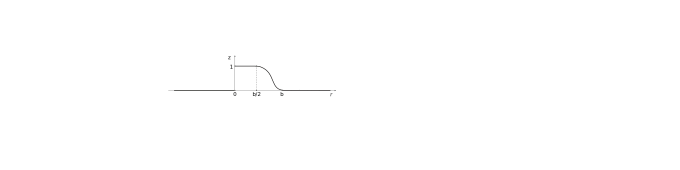
\includegraphics[scale=1.8]{JumpFunction}\\
  \caption{Plot of the function $\zeta$.}\label{FigPlotZeta}
\end{figure}





To prove that $\lambda\in \sigma(\cH)$ is an accumulation point for some sequence $\{\lambda^\eps\}_{\eps>0}\subset \sigma(H_\eps)$, we will apply the method of quasimodes.
Let $A$ be a self-adjoint operator in a Hilbert space $L$.
We say a pair $(\mu, \phi)\in \Real\times \dom A$ is a \textit{quasimode} of  $A$ with the accuracy $\delta$, if $\phi\neq 0$  and
$\|(A-\mu)\phi\|_L\leq\delta\|\phi\|_L$.


\begin{lem}[\hglue-0.1pt{\cite[p.139]{PDEVinitiSpringer}}]\label{LemQuasimodes}
   Assume $(\mu, \phi)$ is a quasimode of $A$ with accuracy $\delta>0$ and  the spectrum of $A$ is discrete in  the interval
$[\mu-\delta, \mu+\delta]$. Then there exists an eigenvalue $\mu_*$ of  $A$ such that $|\mu_*-\mu|\leq\delta$.
\end{lem}
\begin{proof}
If $\mu\in \sigma(A)$, then $\mu_*=\mu$. Otherwise  the distance $d_\mu$ from $\mu$ to the spectrum of $A$  can be computed as
\begin{equation*}
  d_\mu=\|(A-\mu)^{-1}\|^{-1}
  =\inf_{\psi\neq0}\frac{\|\psi\|_L}{\|(A-\mu)^{-1}\psi\|_L},
\end{equation*}
where $\psi$ is an arbitrary vector of $L$. Taking $\psi=(A-\mu)\phi$, we deduce
\begin{equation*}
  d_\mu\leq \frac{\|(A-\mu)\phi\|_L}{\|\phi\|_L}\leq \delta,
\end{equation*}
from which the assertion  follows.
\end{proof}

Given an eigenvalue $\lambda$ of $\cH$ with eigenfunction $u$, we will prove that the pair $(\lambda, v_\eps)$ is a quasimode of $H_\eps$ with an infinitely small accuracy as $\eps\to 0$, where $v_\eps$ is  constructed as in \eqref{AsymptoticsVe} above. Write $\varrho_\eps=(H_\eps-\lambda)v_\eps$.
We see that
\begin{equation*}
 \varrho_\eps=(-\Delta+W-\lambda)( u-\eta_\eps)=\Delta\eta_\eps-W\eta_\eps+\lambda\eta_\eps
\end{equation*}
outside $\omega_\eps$, and therefore $\sup_{x\in\Real^2\setminus \omega_\eps}|\varrho_\eps(x)|\leq c_1\eps$, because of \eqref{EtaEpsEstimate}. Note that $\eta_\eps$ is a function of compact support.



Recalling representation \eqref{LaplacianInSN} of the Laplace operator in the local coordinates, we deduce
\begin{multline*}
-\Delta+W(x)+V_\eps(x)
=-\eps^{-2}\partial^2_n+\eps^{-1}\kappa\partial_n
+n\kappa^2\partial_n-\partial^2_s-\eps P_\eps\\
+W(s,\eps n)+ \eps^{-2}V(n)+\eps^{-1}U(s,n) =\eps^{-2}\ell_0+\eps^{-1}\ell_1+\ell_2+W(s,\eps n)-\eps P_\eps,
\end{multline*}
for $x\in \omega_\eps$, where $\ell_0=-\partial^2_n+V$, $\ell_1=\kappa\partial_n
+U$ and $\ell_2=n\kappa^2\partial_n-\partial^2_s$. Then
\begin{multline}\label{RhoEpsOmegaEps}
  \varrho_\eps=(-\Delta+W+V_\eps -\lambda)v_\eps
  =\big(\eps^{-2}\ell_0+\eps^{-1}\ell_1+\ell_2+W(s,\eps n)-\eps P_\eps-\lambda\big)\big(v_0+\eps v_1+\eps^2 v_2\big)\\
  =\eps^{-2}\ell_0v_0+\eps^{-1}(\ell_0v_1+\ell_1v_0)+\big(\ell_0v_2+\ell_1v_1
  +(\ell_2+W(s,0)-\lambda)v_0\big)
  \\
  +(W(s,\eps n)-W(s,0))v_0+\eps \big(\ell_1v_2+(\ell_2+W(s,\eps n)-\lambda)
  (v_1+\eps v_2) - P_\eps v_\eps\big).
\end{multline}
From our choice of $v_k$, we derive that the first three terms in the right-hand side vanish. Then $\sup_{x\in\omega_\eps}|\varrho_\eps(x)|\leq c_2\eps$. Hence we have
\begin{equation*}
  \|(H_\eps-\lambda)v_\eps\|_{L_2(\Real^2)}=
  \|\varrho_\eps\|_{L_2(\Real^2)}\leq |\omega_{2\beta}|^{1/2}\sup_{\Real^2}|\varrho_\eps|\leq c_3 \eps,
\end{equation*}
since $\supp \varrho_\eps\subset \omega_{2\beta}$.
On the other hand, the main contribution  to the $L_2(\Real^2)$-norm of $v_\eps$ is given by the eigenfunction $u$, because the norms of $\eta_\eps$ and $v_k$, $k=0,1,2$, are infinitely small  as $\eps\to 0$. Therefore $\|v_\eps\|_{L_2(\Real^2)}\geq \frac{1}{2}\|u\|_{L_2(\Real^2)}$ for $\eps$ small enough.
 Finally, we obtain
\begin{equation*}
 \|(H_\eps-\lambda)v_\eps\|_{L_2(\Real^2)}\leq c_3 \eps
 \leq 2c_3 \eps\|u\|_{L_2(\Real^2)}^{-1}\,\|v_\eps\|_{L_2(\Real^2)}\leq c_4 \eps\,\|v_\eps\|_{L_2(\Real^2)}.
\end{equation*}
In view of Lemma~\ref{LemQuasimodes}, there exists an eigenvalue $\lambda^\eps$ of $H_\eps$ such that
\begin{equation*}
  |\lambda^\eps-\lambda|\leq c_4\eps
\end{equation*}
for all $\eps$  small enough.

\vskip60pt

\section{Proof of Main Theorem}
Let $\{\lambda^\eps\}_{\eps>0}$ be a sequence of eigenvalues of operator $H_\eps$ and $\{u_\eps\}_{\eps>0}$ be the sequence of the corresponding eigenfunctions.
Assume that $\|u_\eps\|_{L_2(\Real^2)}=1$.

\begin{lem}
  Assume that $\lambda^\eps\to \lambda$ and $u_\eps\to u$ in $L_2(\Real^2)$ weakly as $\eps\to 0$.

  (i) For any bounded domain $D\subset \Real^2$ such that $\overline{D}\cap\gamma=\emptyset$ the sequence of eigenfunctions $u_\eps$ converges in $W_2^2(D)$ weakly, as $\eps\to 0$, to some function $u$. If potential $W$ belongs to $C^2(\overline{D})$, then $u_\eps\to u$ in $W_2^4(D)$ weakly.

  (ii) The function $u$ solves the equation
  \begin{equation}\label{EqnForUoutside}
  -\Delta u+Wu=\lambda u\quad \text{in } \Real^2\setminus \gamma.
  \end{equation}

  (iii)  For any bounded domain $D\subset \Real^2$ there exists the constant $C$ such that
 \begin{equation}\label{UepsW22OmegaEps}
   \|u_\eps\|_{W_2^2(D\setminus\omega_\eps)}\leq C
 \end{equation}
for all $\eps$ small enough.

 (iv) Finally, $u_\eps|_{\gamma_{-\eps}}\to u^-$ and  $u_\eps|_{\gamma_{\eps}}\to u^+$ in $L_2(\gamma)$ weakly as $\eps\to 0$.
\end{lem}


\begin{proof}
\textit{(i)} Recall that the support of short-range potential $V_\eps$ lies in $\omega_\eps$ and chose $\eps$  so small that $D\cap \omega_\eps=\emptyset$. Then for any $\phi\in C_0^\infty(D)$ we conclude from \eqref{SpectralEqn} that
 \begin{equation*}
    \int_{D} \Delta u_\eps\phi\,dx=\int_{D} (W-\lambda^\eps)\, u_\eps\phi\,dx.
  \end{equation*}
The right-hand side  has a limit as $\eps\to 0$ by the assumptions, thus the left-hand side also converges for all $\phi\in C_0^\infty(D)$, i.e., $\Delta u_\eps\to \Delta u$ in $L_2(D)$ weakly. From this we deduce that $u_\eps$ converges to $u$ in  $W_2^2(D)$ weakly, and hence that
 \begin{equation*}
    \int_{D} \Delta u\phi\,dx=\int_{D} (W-\lambda)\,u\phi\,dx.
  \end{equation*}
If $W\in C^2(D)$, then we can apply the Laplace operator to both sides of equality $\Delta u_\eps=(W-\lambda^\eps)u_\eps$  and obtain
 \begin{equation*}
    \int_{D} \Delta^2 u_\eps\phi\,dx=\int_{D} \big((W-\lambda^\eps)\,\Delta u_\eps\phi+2\nabla W\nabla u_\eps\phi+\Delta W u_\eps\phi\big)\,dx.
  \end{equation*}
The right-hand side of this identity  converges as $\eps\to 0$ for all $\phi\in C_0^\infty(D)$. From this we see that $\Delta^2 u_\eps\to \Delta^2 u$ in $L_2(D)$ weakly, and finally that $u_\eps\to u$ in  $W_2^4(D)$ weakly.

\textit{(ii)} From what has already been proved, we have
  \begin{equation*}
    \int_{\Real^2} \Delta u\phi\,dx=\int_{\Real^2} (W-\lambda)\,u\phi\,dx
  \end{equation*}
for all test functions $\phi\in C^\infty_0(\Real^2)$ such that $\supp \phi\cap\gamma=\emptyset$.
Therefore $u$ is a solution of \eqref{EqnForUoutside}.



\textit{(iii)}
Let $\chi_{\eps}$ be the characteristic function of $D\setminus\omega_\eps$.
We conclude from
 \begin{equation*}
 \int_{D\setminus\omega_\eps} \Delta u_\eps\phi\,dx=\int_{D\setminus\omega_\eps} (W-\lambda^\eps)\,u_\eps\phi\,dx
  \end{equation*}
that the family of functionals $\chi_\eps \Delta u_\eps$ in $L_2(\Real^2)$
is pointwise bounded, since the right-hand side of the last identity converges for any $\phi\in L_2(\Real^2)$. In view of  the uniform boundedness principle, we have $\|\chi_\eps \Delta u_\eps\|_{L_2(\Real^2)}\leq C_1$,
from which \eqref{UepsW22OmegaEps} follows.

\textit{(iv)}
Let us introduce the function
$\zeta_\eps(r)=(r-\eps)\zeta(r)\chi_{(\eps,+\infty)}(r)$,
where $\chi_{(\eps,+\infty)}$ is the characteristic function of $(\eps,+\infty)$ and $\zeta$ is  plotted in Fig.~\ref{FigPlotZeta}.
Since $\zeta_\eps(\eps)=0$ and $\zeta_\eps'(\eps+0)=1$ for $\eps$ small enough, integrating by parts yields
\begin{equation}\label{IntUepsDg}
  \int_{\gamma_\eps} u_\eps a \,d\gamma=\int_{D^+_\eps} (W-\lambda^\eps)u_\eps a\zeta_\eps\,dx-\int_{D^+_\eps} u_\eps \Delta (a\zeta_\eps)\,dx.
\end{equation}
Here $a$ is a smooth function on $\gamma$ and $D^+_\eps=\omega_\beta^+\setminus \omega_\eps$.
Similarly, we obtain from \eqref{EqnForUoutside} the equality
 \begin{equation}\label{IntUDg}
  \int_{\gamma} u^+ a \,d\gamma=\int_{\omega_\beta^+} (W-\lambda)u a\zeta_0\,dx-\int_{\omega_\beta^+} u \Delta (a\zeta_0)\,dx,
\end{equation}
where $\zeta_0(r)=r\zeta(r)$.
Obviously,
\begin{equation*}
   \int_{D^+_\eps} (W-\lambda^\eps)u_\eps a\zeta_\eps\,dx\to
   \int_{\omega_\beta^+} (W-\lambda)u a\zeta_0\,dx
\end{equation*}
as $\eps\to 0$, because $\zeta_\eps$ converges to $\zeta_0$ uniformly on $\Real_+$. Recalling \eqref{LaplacianInSN}, we can write
\begin{multline}\label{IntDelta}
  \int_{\omega_\beta^+}u_\eps \Delta (a\zeta_\eps)\,dx=
  \int_{S} \int_0^\beta u_\eps(s,r)\zeta_\eps(r) \,\partial_s\left(\frac{a'(s)}{1-r \kappa(s)}\right)\,ds\,dr
  \\
  +\int_{S} \int_0^\beta u_\eps(s,r)a(s)\big(J(s,r)(2\zeta'(r)+(r-\eps)\zeta''(r))
  -\kappa(s)(r-\eps)\zeta'(r)\big)\,ds\,dr\\
  -
  \int_{S} \int_\eps^\beta u_\eps(s,r)a(s)\kappa(s)\zeta(r)\,ds\,dr,
\end{multline}
provide $\eps<\beta/2$. Here we used  the equalities $\zeta'(r)=0$ and $\zeta''(r)=0$ for $r\in(0,\eps)$.
The right-hand side of \eqref{IntDelta} converges to
\begin{multline*}
   \int_{S} \int_0^\beta u^+(s,r)\zeta_0(r) \,\partial_s\left(\frac{a'(s)}{1-r \kappa(s)}\right)\,ds\,dr
  \\
  +\int_{S} \int_0^\beta u^+(s,r)a(s)\big(J(s,r)(2\zeta'(r)+r\zeta''(r))
  -\kappa(s)(\zeta(r)+r\zeta'(r))\big)\,ds\,dr,
\end{multline*}
which coincides with $\int_{\omega_\beta^+}u^+ \Delta (a\zeta_0)\,dx$.
Therefore we conclude from \eqref{IntUepsDg} and \eqref{IntUDg} that
$\int_{\gamma_\eps} u_\eps a \,d\gamma\to \int_{\gamma} u^+ a \,d\gamma$ for all $a\in C^\infty(\gamma)$, hence that  $u_\eps|_{\gamma_{\eps}}\to u^+$ in $L_2(\gamma)$ weakly as $\eps\to 0$. The proof of the weak convergence for   $u_\eps|_{\gamma_{-\eps}}$ is similar.
\end{proof}






\subsection{Case of zero-energy resonance}


$\Upsilon=\tfrac12(\theta^2-1)\kappa+\mu$.

\begin{lem}\label{lemConvD}
  Suppose that $\lambda^\eps\to \lambda$ and $u_\eps\to u$ in $L_2(\Real^2)$ weakly as $\eps\to 0$, and   the one-dimensional Schr\"odinger operator~$-\frac{d^2}{d t^2}+V$  possesses a zero-energy resonance, then $\lambda$ is an eigenvalue of $\cH$ associated with the eigenfunction $u$.
\end{lem}


%We have divided the proof into a sequence of propositions.




The eigenvalue $\lambda^\eps$ and the corresponding eigenfunction $u_\eps$ satisfy the identity
\begin{equation*}
   \int_{\Real^2}\big(\nabla u_\eps \nabla \phi+
              (W+V_\eps-\lambda^\eps)u_\eps \phi\big)\,dx=0, \qquad \phi\in W_2^1(\Real^2).
\end{equation*}


Let $\lambda$ and $u$ the eigenvalue and the corresponding eigenfunction of
 $\cH$. Then
\begin{equation*}
   \int_{\Omega^+}\nabla u \nabla \psi\,dx+\int_{\Omega^-}\nabla u \nabla \psi\,dx
   +\int_{\Real^2}(W-\lambda)u\psi\,dx
   +\int_\gamma \Upsilon u^-\phi^-\,d\gamma=0
\end{equation*}
for all functions $\psi$ belonging to the set $\Psi_\theta=\{f\in W_2^1(\Real^2\setminus \gamma)\colon f^+=\theta f^- \text{ on }\gamma\}$.

Given $\psi\in \Psi_\theta\cap \rd{C_b^\infty(\Real^2\setminus \gamma)}$, we construct a sequence $\{\psi_\eps\}_{\eps>0}$ in the space $W_2^1(\Real^2)$ as follows. Suppose $h$ is a half-bound state of $-\frac{d^2}{d t^2}+V$
such that $h(-1)=1$, and
functions $h_1$ and $h_2$ solve the Cauchy problems on the interval $\cI$
\begin{align}\label{ProblemH1}
&-h_1''+Vh_1=0,\quad  h_1(-1)=0, \;\; h_1'(-1)=1;
\\\label{ProblemH2}
& -h_2''+Vh_2=\kappa(s)h'+U(s,\,\cdot\,)h,\quad
h_2(s,-1)=0, \;\; \partial_n h_2(s,-1)=0
\end{align}
respectively. Let us write
\begin{equation*}
  \psi_0^\eps(s,n)=\psi(s,-\eps)\,h(n), \quad
  \psi_1^\eps(s,n)=\partial_r\psi(s,-\eps)\,h_1(n)
     -\psi(s,-\eps)\,h_2(s,n).
\end{equation*}
and set
\begin{equation*}
  \hat{\psi}_\eps(x)=
  \begin{cases}
    \psi(x), & \text{if } x\in \Real^2\setminus \omega_\eps,\\
     \psi_0^\eps(s,\tfrac{r}{\eps})
     +\eps \psi_1^\eps\left(s,\tfrac{r}{\eps}\right)& \text{if } x=(s,r)\in \omega_\eps.
  \end{cases}
\end{equation*}
The function $\psi_\eps$ does not in general belong to $W_2^1(\Real^2)$, because it  has a jump discontinuity on the boundary $\partial\omega_\eps$ composed of two curves $\gamma_{-\eps}$ and $\gamma_{\eps}$. Then $[\hat{\psi}_\eps]_{-\eps}=0$, by construction.  Recalling the function $\zeta$ plotted in Fig.~\ref{FigPlotZeta}, we write
\begin{equation*}
\rho_\eps(x)=
\begin{cases}
  -[\hat{\psi}_\eps]_{\eps}\,\zeta(r-\eps),& \text{if }x=(s,r)\in
  \omega_{2\beta}\setminus \omega_\eps,\\
  \phantom{-}0,& \text{otherwise}.
\end{cases}
\end{equation*}
Finally, we set $\psi_\eps=\hat{\psi}_\eps+\rho_\eps$.
The direct calculations show that $[\psi_\eps]_{\eps}=0$  and, therefore, $\psi_\eps$ belongs to $W_2^1(\Real^2)$.

The first observation of the sequence $\{\psi_\eps\}_{\eps>0}$ is that it converges to $\psi$ in $L_2(\Real^2)$. In fact,  we have  for all $s\in S$
\begin{equation*}
   [\hat{\psi}_\eps]_{\eps}(s)=\psi(s,\eps)-\theta\psi(s,-\eps)-\eps \psi_{1,\eps}(s,1)\\
  =
  \psi(s,+0)-\theta\psi(s,-0)+O(\eps)=O(\eps),
\end{equation*}
as  $\eps\to 0$, since $\psi(s,+0)=\theta\psi(s,-0)$. Hence $\rho_\eps\to 0$  in $L_2(\Real^2)$.








\begin{prop}\label{PropIntomegaEps}
For $\psi\in \Psi_\theta\cap C_b^\infty(\Real^2\setminus \gamma)$, we have
  \begin{align}\label{IntInLocal1}
   &\int_Q (\partial_n u_\eps \partial_n \psi_0^\eps+Vu_\eps \psi_0^\eps)J_\eps\,dn\,ds=\eps \int_Q \kappa u_\eps \partial_n\psi_0^\eps\,dn\,ds,
    \\
   &\begin{aligned}\label{IntInLocal2}
    \int_Q (\partial_n u_\eps&\partial_n \psi_1^\eps+Vu_\eps \psi_1^\eps+Uu_\eps \psi_0^\eps)J_\eps\,dn\,ds=
    \\
    &\int_S \Big(u_\eps(s,-\eps)\partial_r \psi(s,-\eps)\big(1+\eps \kappa(s)\big)
    \\
    &-
    \theta^{-1}u_\eps(s,\eps)\big(\partial_r\psi(s,-\eps)-\Upsilon(s)\psi(s,-\eps)\big)(1-\eps \kappa(s))\Big)\,ds
    \\
&-\int_Q \kappa u_\eps\, \partial_n\psi_0^\eps\,dn\,ds+
\eps\int_Q \kappa u_\eps (\kappa \partial_n\psi_0^\eps- \partial_n \psi_1^\eps)\,dn\,ds.
    \end{aligned}
  \end{align}
  where $J_\eps(s,n)=1-\eps n \kappa(s)$.
\end{prop}
\begin{proof}
 The function $\psi_0^\eps$ solves the equation $-\partial_n^2v+Vv=0$ in $Q$ and $h'(-1)=h'(1)=0$. Then
\begin{multline*}
  0=\int_Q u_\eps(-\partial_n^2\psi_0^\eps+V \psi_0^\eps)J_\eps\,dn\,ds
  =-\int_S\psi(s,-\eps) ( u_\eps J_\eps h')\big|_{n=-1}^{n=1}\,ds
  \\+
  \int_Q (\partial_n u_\eps \, \partial_n \psi_0^\eps+Vu_\eps \psi_0^\eps)J_\eps\,dn\,ds+
  \int_Q u_\eps\,\partial_n J_\eps \,\partial_n \psi_0^\eps\,dn\,ds
  \\=\int_Q (\partial_n u_\eps \, \partial_n \psi_0^\eps+Vu_\eps \psi_0^\eps)J_\eps\,dn\,ds-\eps
  \int_Q \kappa u_\eps\,\partial_n \psi_0^\eps\,dn\,ds,
\end{multline*}
from which \eqref{IntInLocal1} follows.





Since $h(1)=\theta$, the Lagrange identity $(h_1h'-h_1'h)|_{-1}^1=0$ for equation  \eqref{ProblemH1} implies
\begin{equation}\label{h1At1Theta}
  h_1'(1)=\theta^{-1}.
\end{equation}
Multiplying the equation in \eqref{ProblemH2} by $h$ and  integrating by parts twice yield
\begin{equation*}
 (h'h_2-h\,\partial_n h_2)\big|_{-1}^1=\kappa(s)\int_{\cI}hh'\,dn
  +\int_{\cI}U(s,n)h^2(n)\, dn.
\end{equation*}
Recalling \eqref{IntHHpr}, it follows that $\theta \,\partial_n h_2(s,1)=-\tfrac{1}{2}(\theta^2-1)\kappa(s)-\mu(s)$ and finally that
\begin{equation}\label{pdH2IsUpsilon}
\partial_n h_2(s,1)=-\theta^{-1}\Upsilon(s).
\end{equation}
To prove \eqref{IntInLocal2}, we note that $\psi_1^\eps$ is a solution of the equation
\begin{equation*}
-\partial_n^2v+Vv=-\kappa \partial_n \psi_0^\eps-U\psi_0^\eps,
\end{equation*}
which follows from \eqref{ProblemH1} and \eqref{ProblemH2}. Hence
\begin{equation}\label{IntIdenForPsi1}
  \int_Qu_\eps (-\partial_n^2 \psi_1^\eps+V \psi_1^\eps+U \psi_0^\eps)J_\eps\,dn\,ds=-\int_Q \kappa u_\eps\, \partial_n\psi_0^\eps J_\eps\,dn\,ds.
\end{equation}
On the other hand,  integrating by parts with respect to $n$,  we find
\begin{multline}\label{UepsPdPsi1Int}
  -\int_Q u_\eps \,\partial_n^2 \psi_1^\eps J_\eps\,dn\,ds=
  \int_Q \partial_n (u_\eps J_\eps) \,\partial_n \psi_1^\eps\,dn\,ds
  -\int_S(u_\eps J_\eps\partial_n \psi_1^\eps)\big|_{n=-1}^{n=1}\,ds
  \\=
  \int_Q \partial_n u_\eps  \,\partial_n \psi_1^\eps J_\eps\,dn\,ds-
  \eps\int_Q \kappa u_\eps \,\partial_n \psi_1^\eps\,dn\,ds
  \\-
  \int_S\Big(u_\eps(s,\eps n) J_\eps(s,n)\big(\partial_r\psi(s,-\eps)\,h_1'(n)
     -\psi(s,-\eps)\,\partial_n h_2(s,n)\big) \Big)\Big|_{n=-1}^{n=1}\,ds
  \\=
  \int_Q \partial_n u_\eps  \,\partial_n \psi_1^\eps J_\eps\,dn\,ds-
  \eps\int_Q \kappa u_\eps \,\partial_n \psi_1^\eps\,dn\,ds
  \\-
  \int_S \bigg(\theta^{-1}u_\eps(s,\eps)\big(\partial_r\psi(s,-\eps)
    -\Upsilon(s)\psi(s,-\eps)\big)(1-\eps \kappa(s))
    \\
    -u_\eps(s,-\eps)\partial_r \psi(s,-\eps)\big(1+\eps \kappa(s)\big)
\Big)\,ds,
\end{multline}
in view of initial conditions \eqref{ProblemH1}, \eqref{ProblemH2} and equalities \eqref{h1At1Theta},  \eqref{pdH2IsUpsilon}. Substituting
\eqref{UepsPdPsi1Int} into \eqref{IntIdenForPsi1}, we obtain \eqref{IntInLocal2}.
\end{proof}


\begin{prop}
Under the assumptions of Lemma~\ref{lemConvD}, for all $\psi\in \Psi_\theta\cap C_b^2(\Real^2\setminus \gamma)$ we have
  \begin{equation*}
  \int_{\omega_\eps}\big(\nabla u_\eps \nabla \psi_\eps+  V_\eps u_\eps \psi_\eps\big)\,dx\to \int_\gamma \Upsilon u^- \psi^-\,d\gamma,
  \end{equation*}
as $\eps$ tends to zero.
\end{prop}
\begin{proof}
Let us note here, for future use,
\begin{gather*}
 \int_{\omega_\eps} g(x)\,dx=\eps \int_{Q} g(s,\eps n)J_\eps(s,n)\,ds\,dn,
 \\
|\nabla v(x_\eps)|^2=\eps^{-2}|\partial_n v(s,n)|^2+J^{-2}_\eps(s,n )\,|\partial_s v(s,n)|^2,
\end{gather*}
where $v(x_\eps)$ stands for $v(s,\nep)$, cf.  \eqref{ScalarProdGrads}. Then
 \begin{multline*}
     \int_{\omega_\eps}\big(\nabla u_\eps \nabla \psi_\eps+  V_\eps u_\eps \psi_\eps\big)\,dx
     \\
     = \eps^{-1}\int_Q\big( \partial_n u_\eps\, \partial_n \psi_\eps+\eps^2J_\eps^{-2}\partial_s u_\eps \,\partial_s \psi_\eps+ V u_\eps \psi_\eps+\eps U u_\eps \psi_\eps\big)J_\eps \,dn\,ds
     \\
     =\eps^{-1}\int_Q (\partial_n u_\eps \partial_n \psi_0^\eps+Vu_\eps \psi_0^\eps)J_\eps\,dn\,ds
     +\int_Q  (\partial_n u_\eps\partial_n \psi_1^\eps+Vu_\eps \psi_1^\eps+Uu_\eps \psi_0^\eps)J_\eps\,dn\,ds
     \\
     +\eps\int_Q U u_\eps \psi_1^\eps J_\eps\,dn\,ds
     +\eps^2\int_Q \partial_s u_\eps \,\partial_s \psi_\eps J_\eps^{-1} \,dn\,ds.
  \end{multline*}
  In view of Proposition~\ref{PropIntomegaEps}, we have
  \begin{multline}\allowdisplaybreaks
  \label{IntOmegaEpsTo}
     \int_{\omega_\eps}\big(\nabla u_\eps \nabla \psi_\eps+  V_\eps u_\eps \psi_\eps\big)\,dx
     = \int_S \Big(u_\eps(s,-\eps)\partial_r \psi(s,-\eps)\big(1+\eps \kappa(s)\big)
    \\
    -
    \theta^{-1}u_\eps(s,\eps)\big(\partial_r\psi(s,-\eps)-\Upsilon(s)\psi(s,-\eps)\big)(1-\eps \kappa(s))\Big)\,ds
     \\
     +\eps\int_Q u_\eps\big(\kappa^2\partial_n \psi_0^\eps-\kappa\partial_n \psi_1^\eps+U \psi_1^\eps J_\eps\big)\,dn\,ds
     +\eps^2\int_Q \partial_s u_\eps \,\partial_s \psi_\eps J_\eps^{-1} \,dn\,ds.
  \end{multline}
For any sequence $\phi_\eps$ bounded in the $L_2(Q)$-norm,the estimate
\begin{multline*}
  \left|\int_Q u_\eps(s,\eps n) \phi_\eps(s,n) \,dn\,ds\right|\leq
  \left(\int_Q |u_\eps(s,\eps n)|^2\,dn\,ds\right)^{1/2}\|\phi_\eps\|_{L_2(Q)}
  \\
  \leq c\left(\eps^{-1}\int_{\omega_\eps} |u_\eps(x)|^2\,dx\right)^{1/2}
  \leq c\eps^{-1/2}\|u_\eps\|_{L_2(\Real^2)}
  =c\eps^{-1/2}
\end{multline*}
holds. Also, we have
\begin{equation*}
 \left| \int_Q \partial_s u_\eps \,\partial_s \psi_\eps J_\eps^{-1} \,dn\,ds\right|=\left| \int_Q u_\eps \,\partial_s(J_\eps^{-1}\partial_s\psi_\eps ) \,dn\,ds\right|\leq c_1\eps^{-1/2},
\end{equation*}
because $\kappa \in C^1(\gamma)$ and $\psi\in C^\infty_b(\Real^2\setminus \gamma)$ and, therefore, the function $\partial_s(J_\eps^{-1}\partial_s\psi_\eps )$ is bounded on $Q$ uniformly on $\eps$.

Then \eqref{IntOmegaEpsTo} implies
\begin{multline*}
     \int_{\omega_\eps}\big(\nabla u_\eps \nabla \psi_\eps+  V_\eps u_\eps \psi_\eps\big)\,dx
     \\
     \to \int_S \Big(u(s,-0)\partial_r \psi(s,-0)-
    \theta^{-1}u(s,+0)\big(\partial_r\psi(s,-0)
    -\Upsilon(s)\psi(s,-0)\big)\Big)\,ds
     \\
     =\int_\gamma \Big(u^-\partial_r \psi^--
    \theta^{-1}u^+\big(\partial_r\psi^-
    -\Upsilon\psi^-\big)\Big)\,d\gamma=\int_\gamma\Upsilon u^-\psi^-\,d\gamma,
 \end{multline*}
since $\theta^{-1}u^+ = u^-$.
\end{proof}


\begin{prop}
  \begin{equation*}
    \int_{\omega_\eps}|u_\eps|^2\,dx\to 0,\quad\text{as } \eps\to 0
  \end{equation*}
\end{prop}
\begin{proof}
  \begin{equation*}
    w_\eps(s,r)=w_0^\eps\left(s,\nep\right)+\eps w_1^\eps\left(s,\nep\right)
    +\eps^2 w_2^\eps\left(s,\nep\right),
  \end{equation*}
 where $w_0^\eps=u_\eps(s,-\eps)h(n)$, and $w_1^\eps$, $w_2^\eps$ solve the Cauchy problems
 \begin{align*}
  &-\pte^2 w_1^\eps+Vw_1^\eps=(-\kappa\pte -U)w_0^\eps, \quad w_1^\eps(\,\cdot\,,-1)= \pte w_1^\eps(\,\cdot\,,-1)=0;\\
  &\begin{aligned}
  -&\pte^2 w_2^\eps+Vw_2^\eps=-(\kappa\pte +U)) w_1^\eps
  +\big(\partial^2_s-n\kappa^2\partial_n-W(\,\cdot\,,0)+\lambda^\eps\big)w_0^\eps, \\
   &w_2^\eps(\,\cdot\,,-1)= \pte w_2^\eps(\,\cdot\,,-1)=0
  \end{aligned}
\end{align*}
respectively. All functions $w_k^\eps\colon Q\to \Real$ are bounded in $L_2(Q)$ uniformly on $\eps$, because $\lambda^\eps\to \lambda$ and $u_\eps(s,-\eps)\to u(s,-0)$ in $L_2(S)$ weakly and therefore $\|u_\eps(\,\cdot\,,-\eps)\|_{L_2(S)}\leq c$.

Reasoning  as in  \eqref{RhoEpsOmegaEps} we deduce that $w_\eps$ is a solution of the equation
\begin{equation*}
  -\Delta w_\eps+(W+V_\eps-\lambda^\eps)w_\eps=f_\eps\quad \text{in } Q_\eps,
\end{equation*}
where $\|f_\eps\|_{L_2(Q_\eps)}\leq c_1 \eps$. It follows that the difference
$g_\eps=w_\eps-u_\eps$ solves the Dirichlet type boundary value problem
 \begin{gather*}
   -\Delta g_\eps+(W+V_\eps-\lambda^\eps)g_\eps=f_\eps\quad \text{in } Q_\eps, \\
   g_\eps(s,-\eps)=0, \qquad g_\eps(s,\eps)=\theta u_\eps(s,-\eps)-u_\eps(s,\eps)+\eps w_1^\eps(s,1)
    +\eps^2 w_2^\eps(s,1).
 \end{gather*}
 Hence
 \begin{equation*}
   \|g_\eps\|_{L_2(Q_\eps)}\leq c_2(\|f_\eps\|_{L_2(Q_\eps)}+)
 \end{equation*}
\end{proof}

\begin{proof}[Proof of Lemma]
  which may be rewritten as
\begin{equation}\label{IdentityUe}
   \int_{\omega_\eps}\big(\nabla u_\eps \nabla \psi_\eps+
   V_\eps u_\eps \psi_\eps\big)\,dx=
    -\int_{\Real^2\setminus\omega_\eps}\nabla u_\eps \nabla \psi_\eps\,dx- \int_{\Real^2}
              (W-\lambda^\eps)u_\eps \psi_\eps\,dx
\end{equation}
The right-hand side of \eqref{IdentityUe} has a finite limit
\begin{equation*}
  -\int_{\Real^2}\big(\nabla u \nabla \psi+
              (W-\lambda)u \psi\big)\,dx
\end{equation*}
as $\eps\to 0$. In particular, the term $\int_{\Real^2}Wu_\eps \phi\,dx$ converges  for any  $\phi\in \dom H_0$ by the rapidly decay of  eigenfunctions of $H_\eps$ \cite[Ch.3.3]{BerezinShubinBook}. Therefore the left-hand side of \eqref{IdentityUe} also converges as $\eps\to 0$.



\end{proof}

















\begin{thebibliography}{10}
\bibitem{BehrndtExnerHolzmannLotoreichik2017}
Behrndt, J., Exner, P., Holzmann, M.,  Lotoreichik, V. (2017). Approximation of Schrodinger operators with $\delta$-interactions supported on hypersurfaces. Mathematische Nachrichten, 290(8-9), 1215-1248.


\bibitem{BerezinShubinBook} F. A. Berezin, M. A. Shubin,
\textit{The Schr\"{o}dinger equation.} Kluwer Academic
Publishers, 1991.

\bibitem{GolovatyHrynivJPA:2010}
    Yu. D. Golovaty,  R. O. Hryniv.
    \textit{On norm resolvent convergence of Schr\"{o}dinger
    operators with $\delta'$-like potentials.}
   Journal of Physics A: Mathematical and Theoretical \textbf{43} (2010) 155204 (14pp) (A Corrigendum: 2011 J. Phys. A: Math. Theor. \textbf{44} 049802)

\bibitem{Golovaty:2012}
    Yu.~Golovaty.
    \textit{Schr\"{o}dinger operators with  $(\alpha\delta'+\beta \delta)$-like potentials: norm resolvent convergence and solvable models,} Methods of Funct. Anal. Topology (3) \textbf{18} (2012), 243--255.

\bibitem{GolovatyHrynivProcEdinburgh2013} Yu. D. Golovaty and R. O. Hryniv. \textit{Norm resolvent convergence of singularly scaled Schr\"{o}dinger operators and $\delta'$-potentials.} Proceedings of the Royal Society of Edinburgh: Section A Mathematics \textbf{143} (2013),  791-816.

\bibitem{GolovatyIEOT2013}
    Yu. Golovaty, \textit{1D Schr\"{o}dinger Operators with Short Range Interactions: Two-Scale Regularization of Distributional Potentials.} Integral Equations and Operator Theory \textbf{75}(3) (2013),   341-362.


\bibitem{Zolotaryuk08}
    A. V. Zolotaryuk.
    \textit{Two-parametric resonant tunneling across the $\delta'(x)$ potential.}
    Adv. Sci. Lett. {\bf 1} (2008), 187-191.

\bibitem{Zolotaryuk09}
    A. V. Zolotaryuk.
    \textit{Point interactions of the dipole type defined through a three-parametric power regularization.}
    Journal of Physics A: Mathematical and Theoretical {\bf 43} (2010), 105302.

\bibitem{GolovatyJPA:2018}
	Yu. Golovaty.
	\textit{Two-parametric  $\delta'$-interactions: approximation by
 	Schr\"{o}dinger operators with localized rank-two perturbations.}
 	Journal of Physics A: Mathematical and Theoretical \textbf{51}(25) (2018), 255202.

\bibitem{GolovatyIEOT:2018}
	Yu. Golovaty.
	\textit{Schr\"{o}dinger operators with singular rank-two perturbations and point interactions.}
	Integr. Equ. Oper. Theory \textbf{90}:57 (2018).



\bibitem{PDEVinitiSpringer}
Fedoruyk MV, Babich VM, Lazutkin, VF, \dots \& Vainberg, B. R.
(1999). Partial Differential Equations V: Asymptotic Methods for
Partial Differential Equations (Vol. 5). Springer Science \&
Business Media.

\bibitem{Nazarov}\rd{Nazarov}

\bibitem{Perez}\rd{Perez}

\end{thebibliography}

\end{document}

We also have $v_0(s,t)=u^-(s)h(t)=\theta^{-1}u^+(s)h(t)$.

ffgggqy
